\documentclass[journal]{vgtc}                % final (journal style)
%\documentclass[review,journal]{vgtc}         % review (journal style)
%\documentclass[widereview]{vgtc}             % wide-spaced review
%\documentclass[preprint,journal]{vgtc}       % preprint (journal style)

%% Uncomment one of the lines above depending on where your paper is
%% in the conference process. ``review'' and ``widereview'' are for review
%% submission, ``preprint'' is for pre-publication, and the final version
%% doesn't use a specific qualifier.

%% Please use one of the ``review'' options in combination with the
%% assigned online id (see below) ONLY if your paper uses a double blind
%% review process. Some conferences, like IEEE Vis and InfoVis, have NOT
%% in the past.

%% Please use the ``preprint''  option when producing a preprint version
%% for sharing your article on an open access repository

%% Please note that the use of figures other than the optional teaser is not permitted on the first page
%% of the journal version.  Figures should begin on the second page and be
%% in CMYK or Grey scale format, otherwise, colour shifting may occur
%% during the printing process.  Papers submitted with figures other than the optional teaser on the
%% first page will be refused. Also, the teaser figure should only have the
%% width of the abstract as the template enforces it.

%% These few lines make a distinction between latex and pdflatex calls and they
%% bring in essential packages for graphics and font handling.
%% Note that due to the \DeclareGraphicsExtensions{} call it is no longer necessary
%% to provide the the path and extension of a graphics file:
%% 
\includegraphics{diamondrule} is completely sufficient.
%%
\ifpdf%                                % if we use pdflatex
  \pdfoutput=1\relax                   % create PDFs from pdfLaTeX
  \pdfcompresslevel=9                  % PDF Compression
  \pdfoptionpdfminorversion=7          % create PDF 1.7
  \ExecuteOptions{pdftex}
  \usepackage{graphicx}                % allow us to embed graphics files
  \DeclareGraphicsExtensions{.pdf,.png,.jpg,.jpeg} % for pdflatex we expect .pdf, .png, or .jpg files
\else%                                 % else we use pure latex
  \ExecuteOptions{dvips}
  \usepackage{graphicx}                % allow us to embed graphics files
  \DeclareGraphicsExtensions{.eps}     % for pure latex we expect eps files
\fi%

%% it is recomended to use ``\autoref{sec:bla}'' instead of ``Fig.~\ref{sec:bla}''
\graphicspath{{figures/}{pictures/}{images/}{./}} % where to search for the images

\usepackage{microtype}                 % use micro-typography (slightly more compact, better to read)
\PassOptionsToPackage{warn}{textcomp}  % to address font issues with \textrightarrow
\usepackage{textcomp}                  % use better special symbols
\usepackage{mathptmx}                  % use matching math font
\usepackage{times}                     % we use Times as the main font
\renewcommand*\ttdefault{txtt}         % a nicer typewriter font
\usepackage{cite}                      % needed to automatically sort the references
\usepackage{tabu}                      % only used for the table example
\usepackage{booktabs}                  % only used for the table example
\usepackage{verbatim}
\usepackage{amsfonts}
\usepackage{amsmath}
%% We encourage the use of mathptmx for consistent usage of times font
%% throughout the proceedings. However, if you encounter conflicts
%% with other math-related packages, you may want to disable it.

%% In preprint mode you may define your own headline. If not, the default IEEE copyright message will appear in preprint mode.
%\preprinttext{To appear in IEEE Transactions on Visualization and Computer Graphics.}

%% In preprint mode, this adds a link to the version of the paper on IEEEXplore
%% Uncomment this line when you produce a preprint version of the article 
%% after the article receives a DOI for the paper from IEEE
%\ieeedoi{xx.xxxx/TVCG.201x.xxxxxxx}

%% If you are submitting a paper to a conference for review with a double
%% blind reviewing process, please replace the value ``0'' below with your
%% OnlineID. Otherwise, you may safely leave it at ``0''.
\onlineid{0}

%% declare the category of your paper, only shown in review mode
\vgtccategory{Research}
%% please declare the paper type of your paper to help reviewers, only shown in review mode
%% choices:
%% * algorithm/technique
%% * application/design study
%% * evaluation
%% * system
%% * theory/model
\vgtcpapertype{please specify}

%% Paper title.
\title{Isosurface Rendering via Deep Geometric Properties Synthesis}

%% This is how authors are specified in the journal style

%% indicate IEEE Member or Student Member in form indicated below
\author{Neng Shi, Jingyi Shen, and Haoyu Li}
\authorfooter{
%% insert punctuation at end of each item
\item
 Neng Shi, Jingyi Shen, and Haoyu Li are with the Department of Computer Science and Engineering, The Ohio State University. E-mail: {shi.1337, shen.1250, li.8460}@osu.edu.
}

%other entries to be set up for journal
\shortauthortitle{Biv \MakeLowercase{\textit{et al.}}: Global Illumination for Fun and Profit}
%\shortauthortitle{Firstauthor \MakeLowercase{\textit{et al.}}: Paper Title}

%% Abstract section.
\abstract{ InSituNet is helpful in flexible exploration of parameter space for large-scale ensemble simulations. However, it has a limitation that it only supports several predefined visual mappings. We propose a solution, focusing on synthesizing the geometry properties of an isosurface via deep generative networks. After getting the predicted geometry properties, by traditional computer graphics techniques, we can get isosurface or volume rendering results with different shading effects.  
} % end of abstract

%% Keywords that describe your work. Will show as 'Index Terms' in journal
%% please capitalize first letter and insert punctuation after last keyword
\keywords{Deep learning, generative networks, volume rendering}

%% ACM Computing Classification System (CCS). 
%% See <http://www.acm.org/class/1998/> for details.
%% The ``\CCScat'' command takes four arguments.

\CCScatlist{ % not used in journal version
 \CCScat{K.6.1}{Management of Computing and Information Systems}%
{Project and People Management}{Life Cycle};
 \CCScat{K.7.m}{The Computing Profession}{Miscellaneous}{Ethics}
}

%% Uncomment below to include a teaser figure.

%% Uncomment below to disable the manuscript note
\renewcommand{\manuscriptnotetxt}{}

%% Copyright space is enabled by default as required by guidelines.
%% It is disabled by the 'review' option or via the following command:
% \nocopyrightspace


\vgtcinsertpkg

%%%%%%%%%%%%%%%%%%%%%%%%%%%%%%%%%%%%%%%%%%%%%%%%%%%%%%%%%%%%%%%%
%%%%%%%%%%%%%%%%%%%%%% START OF THE PAPER %%%%%%%%%%%%%%%%%%%%%%
%%%%%%%%%%%%%%%%%%%%%%%%%%%%%%%%%%%%%%%%%%%%%%%%%%%%%%%%%%%%%%%%%

\begin{document}

%% The ``\maketitle'' command must be the first command after the
%% ``\begin{document}'' command. It prepares and prints the title block.

%% the only exception to this rule is the \firstsection command
\firstsection{Introduction}

\maketitle

%% \section{Introduction} %for journal use above \firstsection{..} instead
Ensemble simulation \cite{wang2018visualization} is important in scientific visualization. For example, in meteorology, meteorologists often use numerical weather forecast models to generate aggregated simulation data. By disturbing the initial conditions or use different prediction model formulas, the collective simulation data usually consist of a series of data members. For Ensemble data \cite{ahrens2014situ, ahrens2014image}, its large number of data members and a high degree of complexity lead to two problems: (1) a long time for scientists to run the simulation and see the results, (2) I/O bottleneck for storing the raw data. Both problems can influence scientists to effectively analyze and evaluate data. In-situ visualization \cite{bauer2016situ, ma2009situ}, in which the calculation results are not stored but directly processed into images at the computing nodes, can greatly reduce the amount of data stored, transmitted, and post-processed. However, when the raw data is not available, the flexibility of post-hoc analysis would be constrained.  

Recently, with the development of deep generative models, people can generate high-quality images given random noise \cite{goodfellow2014generative} or some semantic prior information \cite{mirza2014conditional}. Specifically, in ensemble visualization, He et al. \cite{he2019insitunet} proposed InSituNet, which is a deep learning-based surrogate model to support parameter space exploration for ensemble simulations that are visualized in situ. InSituNet can generate images of high accuracy, and fidelity. However, it has a limitation that it only allows users to switch among several predefined visual mappings (e.g., transfer functions). The main reason is covering such a joint space of all possible simulation and visualization parameters requires a large number of training images.

This study tries to propose a solution for the limitation, focusing on isosurface, which needs only one scalar value (isovalue) to encode. Our final goal is to train a deep network that can generate geometric properties (e.g., depth, normal maps) of an isosurface given simulation, isosurface, and view parameters. After getting the geometric properties of an isosurface, by traditional computer graphics techniques, for example, deferred shading \cite{deering1988triangle} and depth peeling \cite{zolt2003depthpeel}, we can get isosurface or volume rendering results with different shading effects. Currently, due to the time limitation, we may only focus on isosurface and view parameters, without considering the simulation parameter.  

\section{Related Work}

In this section, we review related work in deep generative models for scientific visualization.

\subsection{Deep Generative Models for Scientific Visualization}

Deep generative models (e.g., PixelRNN \cite{oord2016pixel}, PixelCNN \cite{van2016conditional}, VAE \cite{kingma2013auto}, GAN \cite{goodfellow2014generative}, etc.) have evolved in recent years and have achieved exciting accomplishment. Given the training data, generative models can generate new samples from the same distribution. Among them, Generative adversarial networks \cite{goodfellow2014generative} (GANs) represent the highest achievement, and has been used in various applications, including image generation \cite{karras2017progressive, jin2017towards}, image-to-image translation \cite{isola2017image, zhu2017unpaired}, text-to-image translation \cite{zhang2017stackgan, reed2016generative}, super resolution \cite{ledig2017photo}, and 3D object generation \cite{wu2016learning, gadelha20173d}. 

Scientific visualization researchers increasingly use deep generative models to synthesize the visualization results. Berger et al. \cite{berger2018generative} train a generative model to synthesize volume rendering images, conditioned on viewpoints and transfer functions. He et al. \cite{he2019insitunet} proposed InSituNet, a deep learning-based surrogate model to support parameter space exploration for ensemble simulations that are visualized in situ. Weiss et al. \cite{weiss2019volumetric} train a super-resolution network that can upscale a low-resolution sampling of isosurface depths and normals to a high resolution one. Hong et al. \cite{hong2019dnn} implement a deep neural network that accepts original images with goal rendering effect and new viewing parameters as the inputs and synthesizes new images. Some other researchers focus on directly synthesize 3D data. To address a spatial super-resolution problem, Xie et al. \cite{xie2018tempogan} propose a temporally coherent generative model to generate high-resolution fluid flows. Han et al. \cite{han2019tsr} achieve temporal super-resolution of time-varying data by a recurrent generative network (RGN, a combination of RNN and GAN).

Our work is closely related to InSituNet \cite{he2019insitunet}, which focus on parameter space exploration. The difference between our work and InSituNet is that we focus on synthesize the  geometric properties (e.g., depth,normal maps) of an isosurface, rather than visualization images. This idea is similar with the super-resolution work by Weiss et al. \cite{weiss2019volumetric}. 

\section{Isosurface Learning}

\begin{figure*}
  \centering
  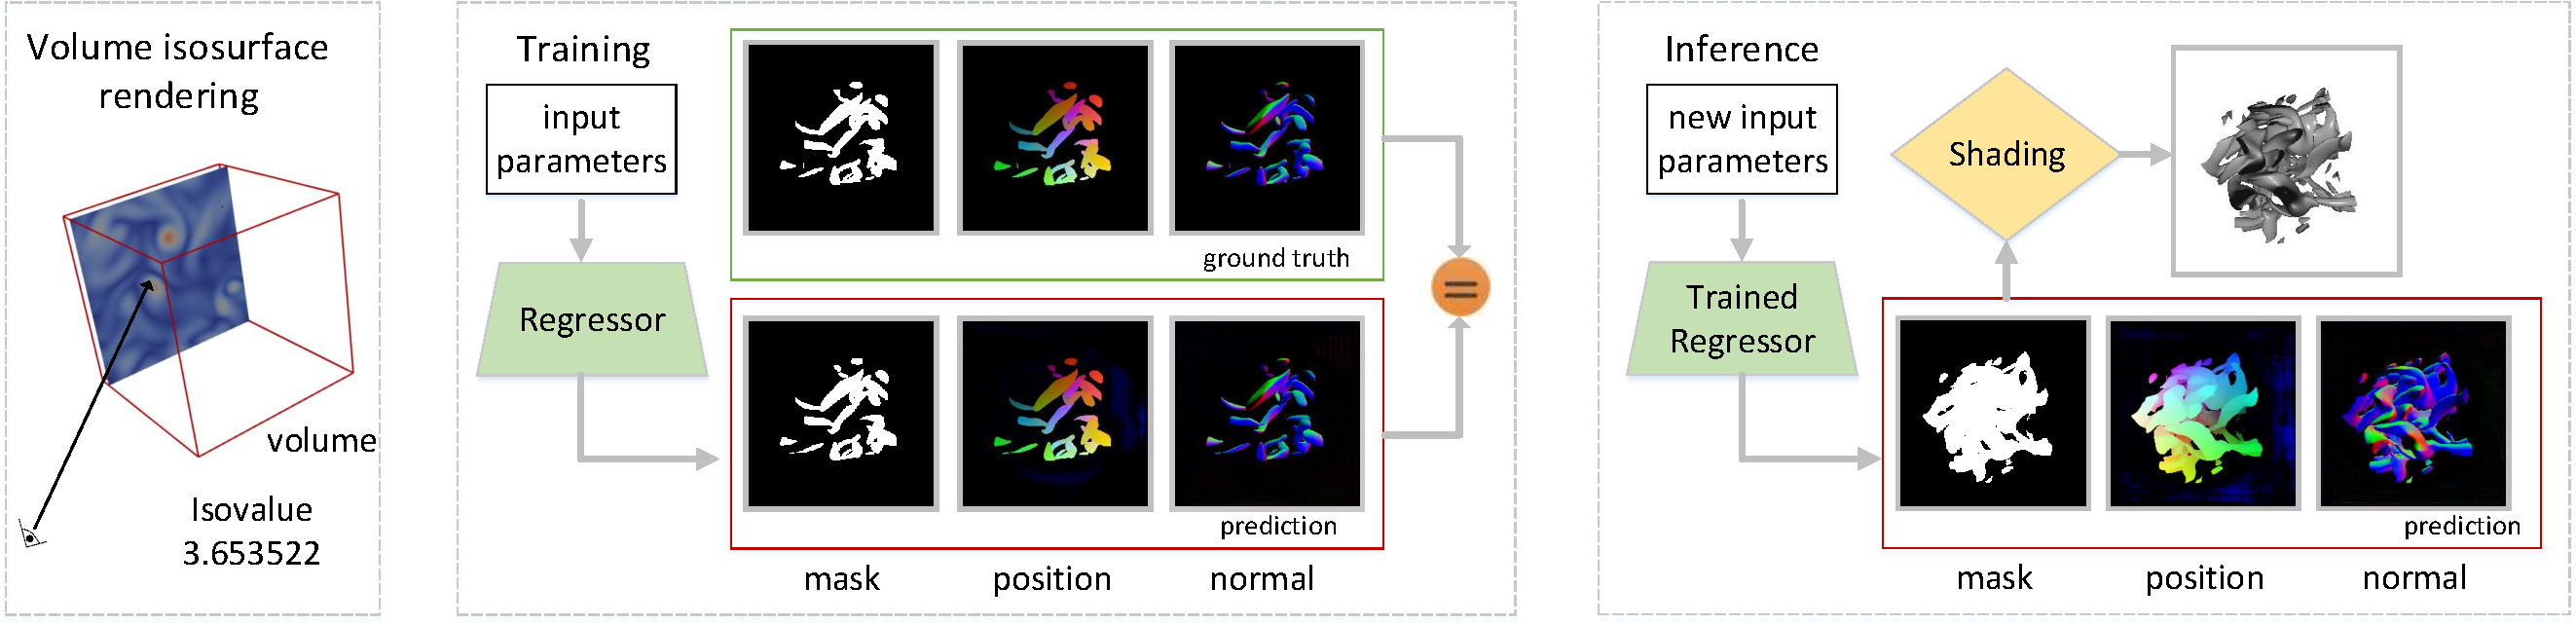
\includegraphics[width=\linewidth]{overview}
  \caption{The Deep Geometric Properties Synthesis Pipeline. For the input volume (vortex in this example), we apply the volumetric ray-casting algorithm with the isovalue and viewpoint as input parameters to generate the training datasets (corresponding geometric properties of an isosurface). The regressor training process takes the input parameters to predict the corresponding geometric properties of an isosurface, and the parameters of the regressor are optimized by minimizing the difference between the predicted geometric properties and the ground truth. Finally, the trained regressor can be used to take new input parameters and predict the corresponding geometric properties of an isosurface. On top of them, deferred shading can be used to generate the final visualization image. }
	\label{fig:overview}
\end{figure*}

As shown in Fig.~\ref{fig:overview}, our deep geometric properties synthesis pipeline consists of three major parts. The first part is about the training data generation. Since we do not consider simulation parameters, we use volume data available online in large volume collections. Then, given the isovalue and viewpoint, we can to implement volumetric ray-casting to generate corresponding geometric properties of an isosurface. Second, with the collected pairs between parameters and the corresponding geometric properties, we train a regressor $R$ to learn the mapping from input parameters to geometric properties. The loss function is used to penalize the difference between the predicted geometric properties and the ground truth ones. We investigate networks trained with different loss functions and analyze the synthesis quality of these networks on the new input parameters that the network has never seen before during the training phase. Third, we do screen-space shading based on the synthesized geometric properties. We can control the lighting conditions and get some interesting visual effects such as shadow maps.

\subsection{Input Data}
We first discuss the two group of input parameters (the isovalue and viewpoint) in detail:

\paragraph{Isovalue}
An isosurface is a surface that represents points of a constant (e.g. pressure, temperature, velocity, density) within a volume of space. The constant controls which isosurface will be computed is called isovalue. By sweeping the isovalue within the defined ranges, people can generate different isosurfaces. 

\paragraph{Viewpoint}
In our experiment, we assume that all the viewpoints are on the viewing sphere \cite{Ji2006DVS}, the center of which is located at the volume center. We can parameterize the viewpoint as a tuple $(\theta, \phi)$ of camera parameters, where $\theta \in [0, 360]$ is the azimuth (longitude) angle and $\phi \in [-90,90]$ is the elevation (latitude) angle. 

Given the isovalue and viewpoint, we implement volumetric ray-casting to get the corresponding geometric properties of an isosurface. We let the ray from the viewpoint advance through the volume until reaching a sample whose intensity is greater than or equal to the threshold value, meaning that we hit the isosurface. Once we find a point belonging to the isosurface, instead of directly applying an illumination model to perform shading, we use the geometry pass in deferred shading \cite{deering1988triangle} to store all kinds of geometric properties in a collection of textures called the G-buffer. In our study, these geometric properties are maps of size $ H \times W $, including:

\begin{itemize}
\item $M^{GT} \in [0, 1] ^ {H \times W}$: The mask binary map in which 1 is for foreground and 0 otherwise. After the network training, it will learn a continuous value, and we will use it to blend the final color over the background.  

\item $N^{GT} \in [-1, +1] ^ {3 \times H \times W}$: The normal map with the normal vectors in the view space.

\item $P^{GT} \in [0, 1] ^ {3 \times H \times W}$: The position map with the position vectors in the local space. We choose the local space position because it is already normalized within the range $[0, 1]$.

\end{itemize}

We concatenate all the geometric properties. Thus, the ground truth geometric property map can be written as $O^{GT} = \{M^{GT}, N^{GT}, P^{GT}\} \in \mathbb{R}^{7 \times H \times W}$. Once the regressor is trained, it can synthesize a new geometric property map $O^{est} = \{M^{est}, N^{est}, P^{est}\} \in \mathbb{R}^{7 \times H \times W}$ from new input parameters. 

\subsection{Network Training}

\begin{figure}
  \centering
  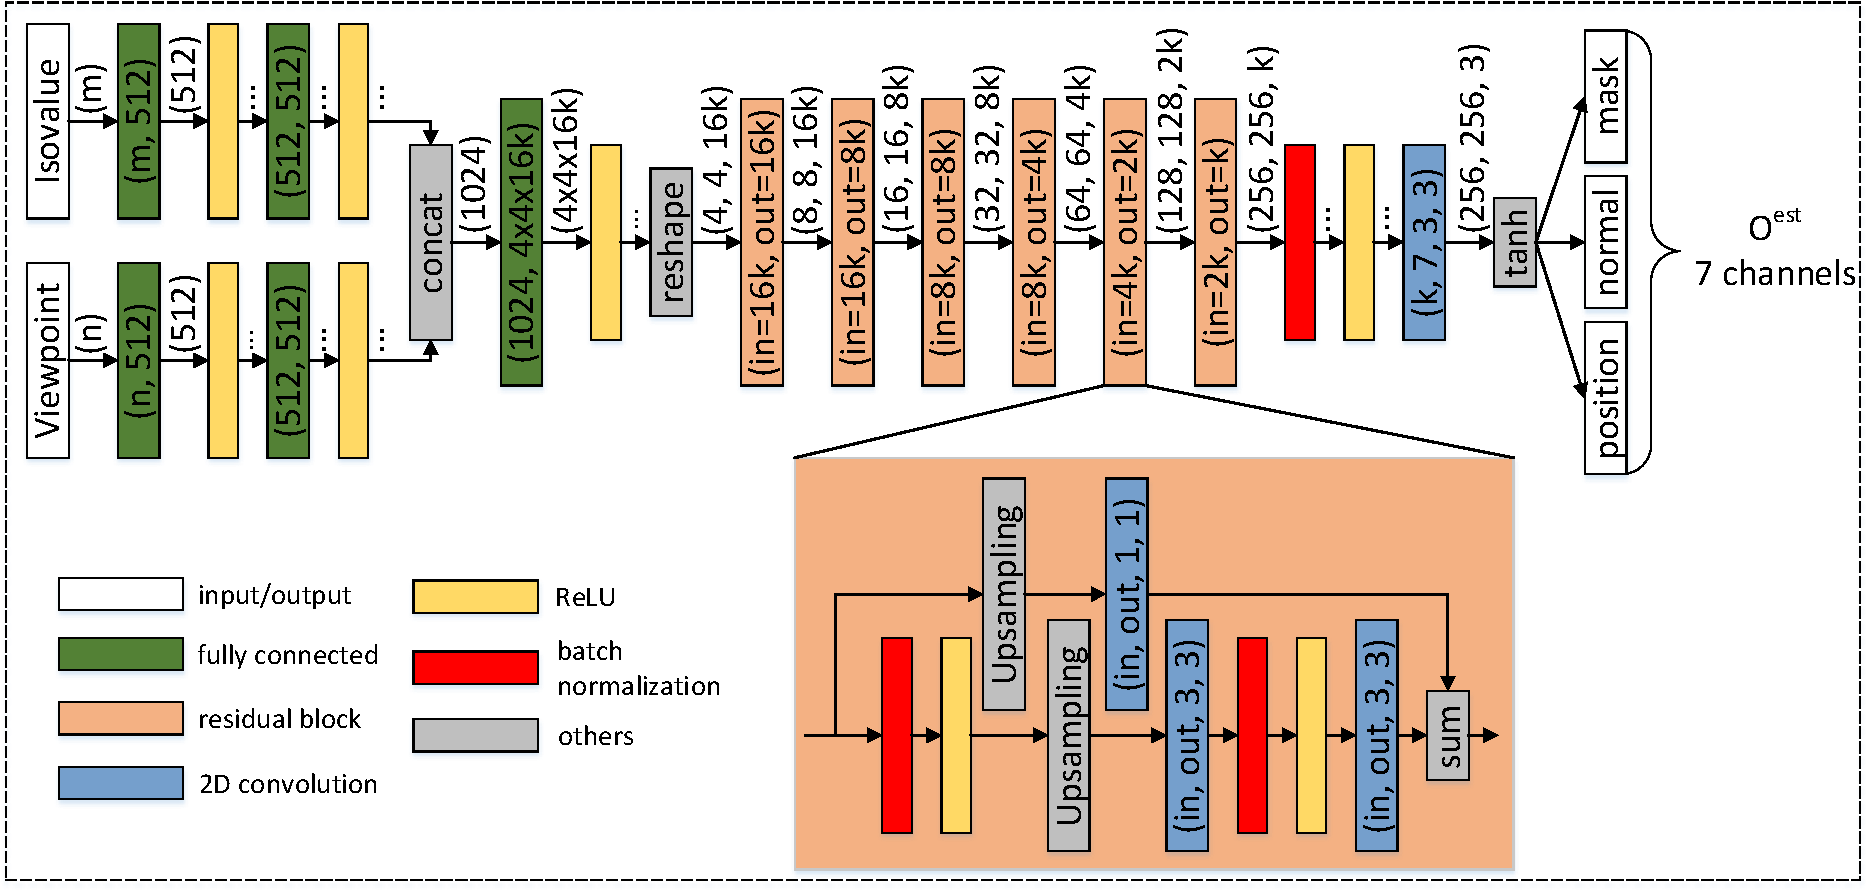
\includegraphics[width=1\linewidth]{regressor}
  \caption{The structure of our regressor $R$. First, it encodes the input parameters into a latent vector. Then the latent vector is projected to a small spatial extent convolutional representation with many feature maps. Next, $6$ residual blocks and the following convolution layer convert this high-level representation a $256 \times 256 \times 7$ pixel map. As InSituNet, the hyperparameter k controls the size of $R$. Specifically, it controls the number of convolution kernels in the intermediate layers.}
  \label{fig:regressor}
\end{figure}

\subsubsection{Network architecture}
We build the regressor following InSituNet proposed by He et al. \cite{he2019insitunet} since our geometric property synthesis problem is similar to their image synthesis problem. Specifically, we train a regressor $R$ whose goal is to encode input parameters (the isovalue and viewpoint) and generate the corresponding geometric properties (mask, position and normal maps). We use one regressor to learn the mapping to all the geometric properties since sharing network parameters until the last layer can help the generated geometric properties match each other.

The structure of the regressor is illustrated in Fig.~\ref{fig:regressor}. The modifications we have performed are concerning the input and output, the other parts of the network are kept unchanged. It takes the isovalue and viewpoint as inputs and outputs a mask map $M^{est}$, a normal map $N^{est}$, and a position map $P^{est}$. The network first separately encodes the two types of input parameters into two latent vectors. Then it concatenates the two latent vectors and encodes them into a new latent vector by another fully connected layer. Second, the latent vector is projected to a small spatial extent convolution representation with many feature maps. What the network do next is super-resolution. The feature map comes through $6$ residual blocks, each of which performs a $2 \times$ super-resolution. For each residual block, it first upsamples the input feature map by nearest neighbor upsampling, then the upsampled feature map is fed into two convolution layers with kernel $3 \times 3$. The residual network relies on the upsampling and $1 \times 1$ convolution in the skip connection whenever the resolution or number of channels need to change. In the last convolution layer, there are 7 convolution kernels, each of which is responsible for generating one output channel. In all layers, the activation functions in the regressor are rectified linear unit (ReLU) except for the output layer, which instead is a tanh to ensure all the channels have pixels in the range $[-1, 1]$.
As InSituNet, we also introduce a hyperparameter $k$ in the network structure to control the network learning capacity by changing the number of convolution kernels in the intermediate layers. Since the geometric properties give much richer information than visualization images, in our experiment, the demand for the network learning capacity is higher, i.e., the hyperparameter $k$ is bigger than the one used in InSituNet. 

\subsubsection{Loss Function}
\label{subsubsection:loss}

We describe the loss function used during training the network. The loss function is used to penalize the difference between the predicted geometric properties and the ground truth ones, which is very important during the geometric properties synthesis.  Different loss functions exert different effects on the synthesized geometric properties and final visualization images.  For example, in our work, some loss functions focus on the global structure, and others concentrate on preserving shape details. Thus, for different rendering goals, We use a different combination of loss functions below. i.e., Our final loss function is a weighted sum of the loss functions below, and for different rendering goals, the coefficient for each loss function varies.    

\paragraph{Per-pixel Normal and Position Loss}

For the first two terms, we consider the per-pixel differences between the synthesized normals and positions. Specifically, $l_1$ loss is employed for both normals and positions. The normal and position losses are only  calculated for pixels marked as foreground in the ground-truth, while other areas that are masked out do not contribute to the loss: 

\begin{alignat}{2}
L_{N} = (\|N^{est} - N^{GT}\|_1) M^{GT}, \\ 
L_{P} = (\|P^{est} - P^{GT}\|_1) M^{GT}.
\end{alignat}

Note that other losses with regular vector norms can be used for penalizing depth and normal differences. For example, $l_2$ distance can be another option, but this tends to generate less sharp maps. 

\paragraph{Mask loss}
During screen-space shading in the third step of the Deep Geometric Properties Synthesis pipeline (see~\ref{subsection:shading}), we only need to calculate the color for foreground regions. Other regions where the mask equals 0 are directly set to the background color. Thus, the network should not care about the position or normal in these areas:

\begin{equation}
L_{M} = \|M^{est} - M^{GT}\|_1.
\end{equation}

We reflect this in the per-pixel normal and position loss, which is a crucial step for simplifying the network's task. Besides, we need to generate a predicted mask map, and we also use $l1$ distance to penalize the difference between predicted and ground-truth mask. 

\paragraph{Adversarial loss}
Lastly, we can penalize structural differences in the output maps concerning ground-truth through an "adversarial" network. During the regressor $R$ training process, a discriminator network $D$ is trained parallel to differentiate ground truth maps and synthesized maps using the technique of \cite{goodfellow2014generative}. Hopefully, once we finish training, the discriminator and the regressor would reach a Nash equilibrium, and at that time, the regressor can generate maps with finer details. 

\begin{figure}
  \centering
  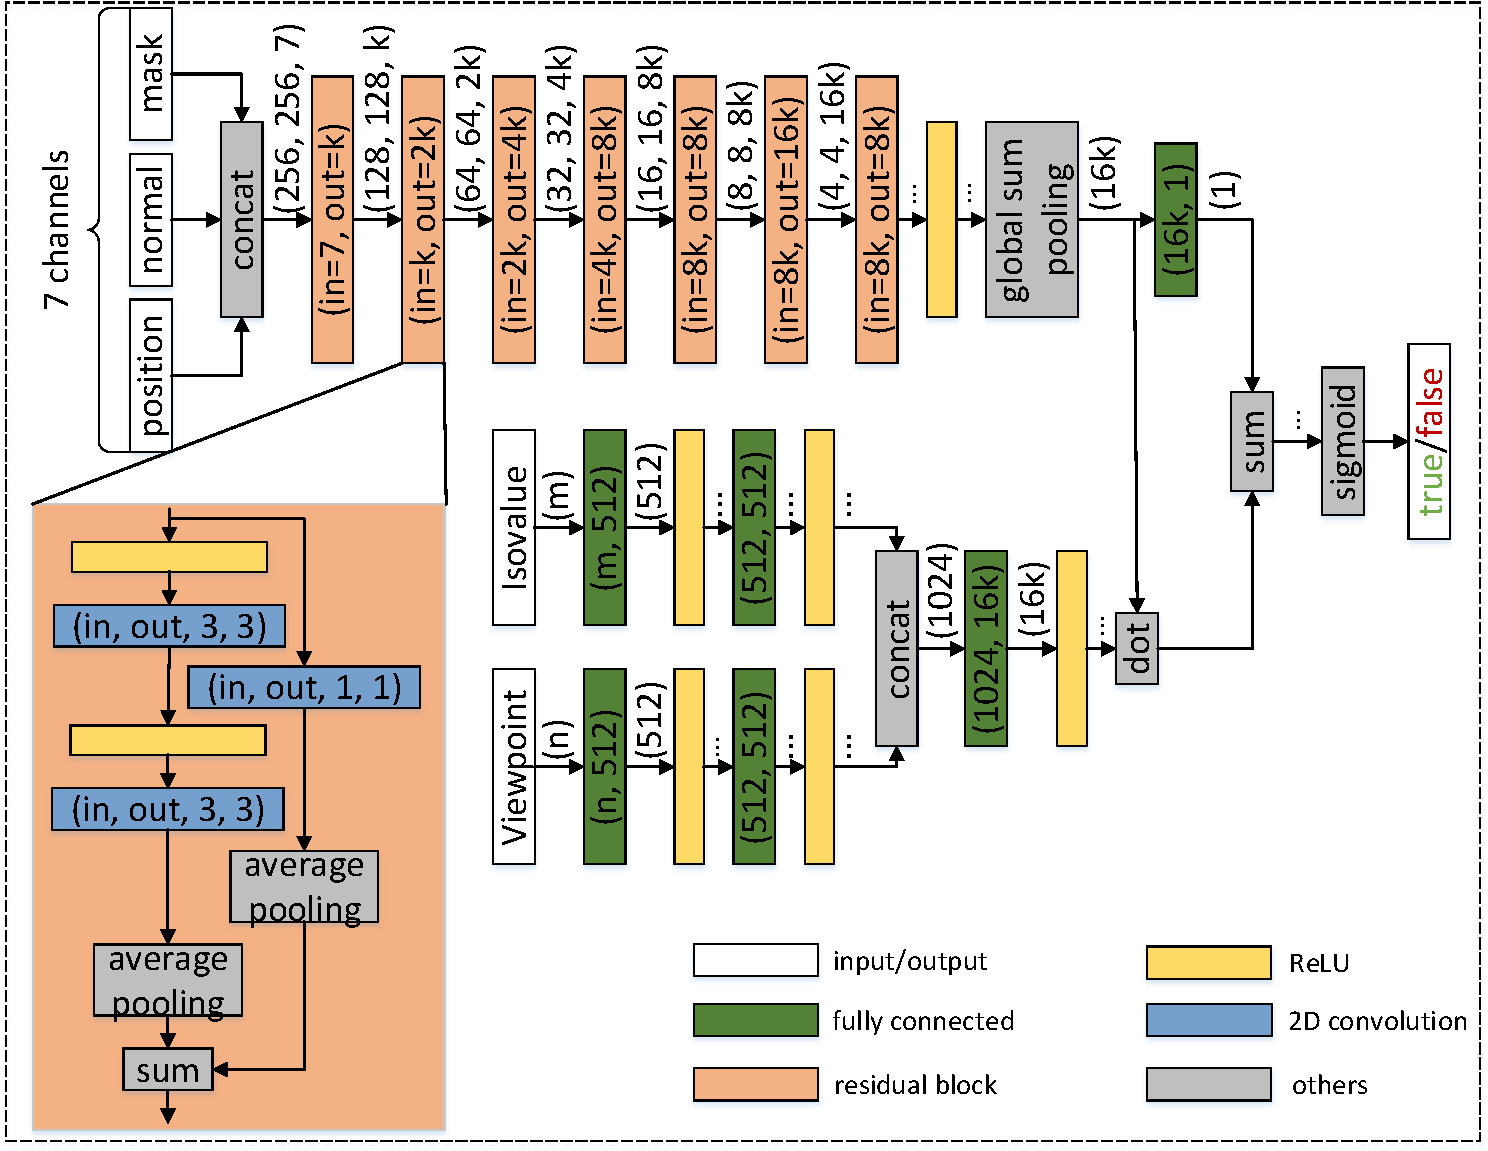
\includegraphics[width=1\linewidth]{discriminator}
  \caption{The structure of our discriminator $D$. Geometric property maps and input parameters are transformed into two latent vectors separately by residual blocks and fully connected layers. Then they are incorporated to get a likelihood value indicating whether the Geometric property map is ground truth or not. Similar to $R$, a hyperparameter k controls the network learning capacity. }
  \label{fig:discriminator}
\end{figure}

We would like to first introduce the structure of the discriminator $D$, which is shown in Fig.~\ref{fig:discriminator}. Similar to regressor $R$, We build the discriminator $D$ following InSituNet, and the modifications we have performed are concerning the input. The discriminator takes a 7-channel map $O$ that concatenates the mask channel, the 3 normal channels, and the 3 position channels as input. Then the input map goes through several residual blocks and is transformed into a latent vector as its feature representation. Meanwhile, several fully connected layers encode the two types of parameters (the isovalue and viewpoint) into another latent vector. The projection-based condition method \cite{miyato2018cgans} is employed to incorporate the two latent vectors. In all layers, the activation functions are ReLU except for the last layer, which instead is a sigmoid function to get a likelihood value within $[0, 1]$.

The loss function we used is the standard binary cross entropy loss in \cite{goodfellow2014generative}. For the generator (regressor $R$), the loss is:

\begin{equation}
L_{adv\_R} = -log(D(O^{est})), 
\end{equation}
By minimizing which, the generator (regressor $R$) is going to fool the discriminator by generating real-look maps. The adversarial loss for the discriminator is defined as:

\begin{equation}
L_{adv\_D} = -log(D(O^{GT}))-log(1-D(O^{est})), 
\end{equation}
by minimizing which, the discriminator is going to distinguish between real and fake maps. 

\subsection{screen-space shading}
\label{subsection:shading}
After getting predicted geometric properties, we employ screen-space Phong shading as a post-processing step. i.e., we render a screen-filled quad and calculate the scene's lighting for each fragment using the geometrical information predicted by the regressor. For a pixel, given a single spotlight source, the final color is calculated by the formula:

\begin{equation}
C_{rgb} = Phong(k_a, k_d, k_s, \alpha, P_{light},  I_{light}, N^{est}, P^{est}), \label{equ:phong}
\end{equation}
with ambient reflection constant $k_a$, diffuse reflection constant $k_d$, specular reflection constant $k_a$,  shininess constant $\alpha$, light source position $P_{light}$, light intensity $I_{light}$, fragment normal $N^{est}$ and fragment position $P^{est}$ as parameters.

The regressor also generates a mask map $M^{est}$ as output. The pixel value in predicted mask map are within the range $[0, 1]$, which shows a smooth fall-off values across edges and allows the network to smooth out edges via

\begin{equation}
C^{est} = lerp(c_{bg}, C_{rgb}, M^{est}), \label{equ:smooth}
\end{equation}

with the background color $c_{bg}$ and fragment mask $M^{est}$ as parameters. 

In (\ref{equ:phong})(\ref{equ:smooth}), despite fragment mask, normal and position, all the other parameters can be set by users. Thus, users can change the lighting conditions to better visualize the feature they are interested in.

\begin{figure*}
  \centering
  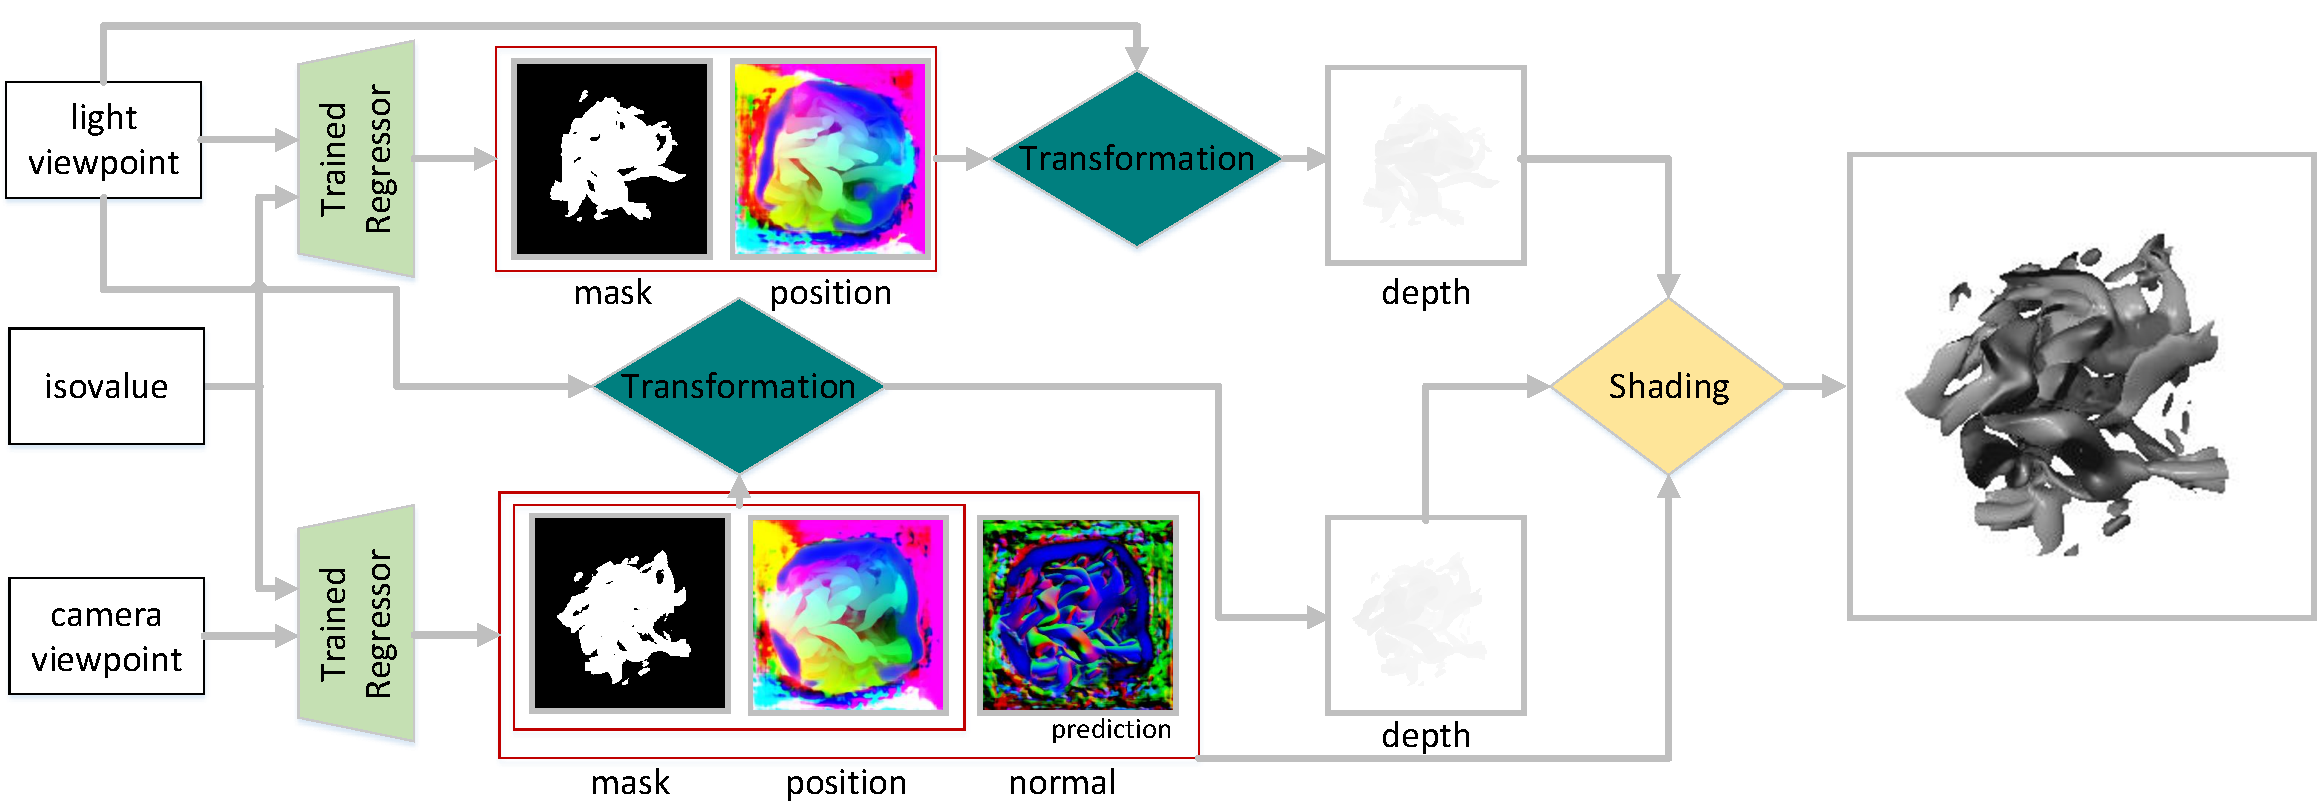
\includegraphics[width=0.8\linewidth]{shadowMap}
  \caption{shadowMap}
  \label{fig:shadowMap}
\end{figure*}

We also employ some advanced lighting effects to add realism to the isosurface rendering scene. For example, Shadows are a result of the absence of light due to occlusion. With shadows, it would become much more apparent how different parts of the isosurface relate to each other.
We generate visualizations images with shadows with the help of the shadow mapping \cite{williams1978casting} technique, and the pipeline is illustrated in Fig.~\ref{fig:shadowMap}. To render an image with shadows, besides the geometric properties needed in the regular deferred shading process, we also need geometric properties from the light's perspective. Generally speaking, to get geometric properties from the light's perspective, we need to train a new regressor because the setting of the light's perspective (e.g., location, projection type, near and far plane) is usually different from the one of camera's perspective. However, we can add some constraints to the light. i.e., if we employ a spotlight whose position is precisely on the viewing sphere and the light points to the volume center, we can simply use the trained regressor to predict the geometric properties needed for the shadow map generation. That is why in Fig.~\ref{fig:shadowMap}, we use the same trained regressor for both the light viewpoint and camera viewpoint. The shadow map stores the closest depth as seen from the light's perspective, which is obtained from the predicted mask and local space position after processing some transformations: 

\begin{equation}
\begin{aligned}
P_{l, lightSpace}^{est} = M_{LightProjection} \times M_{LightView} \times M_{Model} \times P_l^{est}, \\
D_{l, lightSpace}^{est} = P_{l, lightSpace}^{est}.z / P_{l, lightSpace}^{est}.w, \\
S_{l}^{est} = lerp(1.0, D_{l, lightSpace}^{est}, M_{l}^{est}). 
\label{equ:shadowMap}
\end{aligned}
\end{equation}
In the formula above, $P_{l, lightSpace}^{est}$ and $M_{l}^{est}$ are directly predicted from the trained regressor given the isovalue and light viewpoint. $ M_{Model}$ is a matrix which transforms the local space position to world space position. $M_{LightView}$ and $ M_{LightProjection}$ are light space transformation matrices. $P_{l, lightSpace}^{est}$ is the 4-dim light space position, and we get the depth from from the light's perspective $D_{l, lightSpace}^{est}$ simply by dividing the $z$ component by the $w$ component. The final shadow map is obtained by masking out areas with help of $M_{l}^{est}$.      

The next step is to check for every fragment, whethter it is in shadow or not. 

\begin{equation}
\begin{aligned}
P_{lightSpace}^{est} = M_{LightProjection} \times M_{LightView} \times M_{Model} \times P^{est}, \\
projCoords = P_{lightSpace}^{est}.xyz / P_{lightSpace}^{est}.w, \\ 
closetDepth = texture(S_{l}^{est}, projCoords.xy), \\
currentDepth = projCoords.z, \\
shadow = currentDepth > closestDepth.
\end{aligned}
\end{equation}
In the formula above, $P^{est}$ is directly predicted from the trained regressor given the isovalue and camera viewpoint. $P_{lightSpace}^{est}$ is the 4-dim light space position, and similar to \ref{equ:shadowMap}, we transform the Homogeneous coordinate to a Cartesian Coordinate by doing perspective divide. We use $projCoords$ to sample $S_{l}^{est}$, which gives us the closest depth from the light's point of view. The current depth at this fragment from the light's perspective is obtained by retrieving $projCoords.z$. The actual comparison is then simply a check whether $currentDepth$ is higher than $closestDepth$, and if so, the fragment is in shadow, and it would not get the contribution from diffuse and specular light. 

\section{Results}
We evaluated our Deep Geometric Properties Synthesis using the vortex dataset. from four aspects: (1) providing dataset and training process details; (2) evaluating the influence of different hyperparameters;  (3) comparing with the baseline.

\subsection{Dataset and Training Process}
We experiment using the vortex dataset. It has been widely used in feature extraction and tracking. The dataset comes from a pseudo-spectral simulation of vortex structures. The dimensions the dataset is $128 \times 128 \times 128$. The isovalue $I \in [1.214, 7.284]$ (10th and 60th percentiles of the scalar field data range). We sample $9600$ parameter settings from the isovalue-viewpoint joint spaces and employ volumetric ray-casting to generate their corresponding geometric properties as the training dataset. The volumetric ray-casting is implemented in C++, OpenGL and GLSL. The resolution of output geometry property maps is $256 \times 256$.   

The network is implemented in PyTorch \cite{paszke2019pytorch}, and trained with an NVIDIA V100 GPU. We scale all the output geometry maps to $[-1, 1]$ since the value range of the final activation function tanh is $[-1, 1]$.   

The losses for training different networks are obtained by using different weighted combinations of the individual losses introduced in Section \ref{subsubsection:loss}. Table \ref{table:loss} illustrates the specific weight combinations that are used for the networks we have analysed in our work.  

\begin{table}
\caption{Networks and their specific loss function configurations, where $\lambda$ is the weight for $L_{adv\_R}$.}
    \centering
    \begin{tabular}{l|l}
        Network & Losses \\  \hline
        $L_1-geometry$ & $L_M + L_n + L_P$  \\ \hline
        GAN & $L_M + L_n + L_P + \lambda L_{adv\_R}$ \\ 
    \end{tabular}
    \label{table:loss}
\end{table}

For optimization, we initialize parameters in the network using the orthogonal
initialization \cite{saxe2013exact} and apply Adam optimizer \cite{kingma2014adam} to update the parameters. The learning rate for the the regressor $R$ is $5 \times 10^{-5}$. $\beta_1 = 0$, $\beta_2 = 0.999$. With the network "GAN", a different learning rates is set for the discriminator $D$ compared with $R$ to reduce training time and stabilize the training process \cite{roth2017stabilizing}. The learning rate for $D$ is $2 \times 10^{-4}$. 

\subsection{Model Evaluation for Different hyperparameters }

\subsection{Comparison with the Baseline}




\section{Conclusion}
In this work, we propose a Deep Geometric Properties Synthesis method for Isosurface Rendering on top of InSituNet. The trained regressor can generate isosurface rendering images under a single headlight with much better quality than the baseline. And to some extent, we solve the problem in InSitu that it only allows users to switch among several predefined visual mappings by supporting random lighting conditions and shadow effects. 

In the future, we would like to actually run the simulation and apply our method to the simulation data. We would also implement the depth peeling rendering technique to blend different isosurfaces and get volume rendering results that support the change of transfer functions. We also plan to try more loss functions such as Perceptual losses based on the pre-trained VGG network \cite{gatys2016image} to further improve our generation results. 

%\bibliographystyle{abbrv}
\bibliographystyle{abbrv-doi}
%\bibliographystyle{abbrv-doi-narrow}
%\bibliographystyle{abbrv-doi-hyperref}
%\bibliographystyle{abbrv-doi-hyperref-narrow}

\bibliography{template}
\end{document}

